% First comes an example EPS file -- just ignore it and
% proceed on the \documentclass line
% your LaTeX will extract the file if required
\begin{filecontents*}{example.eps}
%!PS-Adobe-3.0 EPSF-3.0
%%BoundingBox: 19 19 221 221
%%CreationDate: Mon Sep 29 1997
%%Creator: programmed by hand (JK)
%%EndComments
gsave
newpath
  20 20 moveto
  20 220 lineto
  220 220 lineto
  220 20 lineto
closepath
2 setlinewidth
gsave
  .4 setgray fill
grestore
stroke
grestore
\end{filecontents*}

\RequirePackage{fix-cm}

%\documentclass{svjour3}                     % onecolumn (standard format)
%\documentclass[smallcondensed]{svjour3}     % onecolumn (ditto)
\documentclass[smallextended,referee]{svjour3}       % onecolumn (second format)
%\documentclass[twocolumn]{svjour3}          % twocolumn
%
\smartqed  % flush right qed marks, e.g. at end of proof
%\usepackage{mathptmx}      % use Times fonts if available on your TeX system


%\documentclass[preprint,review,12pt]{elsarticle} ELSEVIER

\usepackage{epsfig}
\usepackage{natbib}
\usepackage{subfigure}
\usepackage[]{graphicx}
\usepackage{rotating}
\usepackage{here}
\usepackage{calc}
\usepackage{multirow}
\usepackage{amsfonts}
\usepackage{amssymb}
\usepackage{color}
\usepackage{nomencl}
\usepackage{textcomp}
\usepackage{eurosym}
\usepackage[ansinew]{inputenc}
\usepackage[bookmarks=true,bookmarksnumbered=true]{hyperref}

\graphicspath{{figures/EPS/}}


\begin{document}
% \tableofcontents
% \begin{frontmatter}	ELSEVIER

%=====================================================================================
\title{Stability analysis for free surface flows.}
\titlerunning{Stability analysis for free surface flows.}        % if too long for running head
\author{J.M. Gimenez \and L. M. Gonz\'{a}lez}

\institute{ L. M. Gonz�lez \at
           Naval Architecture Department (ETSIN)\\
           Technical University of Madrid (UPM)\\
           Arco de la Victoria s/n, 28040 Madrid, Spain}

\date{Received: date / Accepted: date}
% The correct dates will be entered by the e

\maketitle

%=====================================================================================
\begin{abstract}

This Letter describes how the results of a global stability analysis of a classical circular cylinder are affected when the cylinder submerged and a two phase flow is present. The two phase flow has been transformed into a single phase fluid with variable density and viscosity using a volume of fluid (VOF) characterization. The Navier-Stokes equations which depend on both the Reynolds and Froude numbers, have been fixed to create a particular scenario for the stability analysis. Consequently, the baseflow obtained by the Navier-Stokes equations have been analyzed and the Hopf bifurcation has been obtained for a particular Froude number. The critical Reynolds number and the frequency of the unstable mode have been compared to the classical solution without free surface.

\end{abstract}

%=====================================================================================
\section{Introduction}
\label{S:Intro}
%=====================================================================================

The interaction between the viscous wake of a submerged object and the free surface position is a problem that deserves a serious study. Several reasons sustain this importance, \cite{Dimas} justifies the study due to its potential relevance for the remote sensing of the ocean surface from satellites while \cite{Reichl,Bouscasse} also underline its application to the design of offshore structures and vessels.
It is well known that in the absence of free surface the von Karman vortex street generated by flow past an infinitely long circular cylinder produces a two dimensional time periodic flow for Reynolds numbers between approximately 47 and 189 [1, 2, 3, 4]. The Reynolds number is quantified as $Re= U_\infty D/\nu$ , where $U_\infty$ the fluid velocity far from the cylinder, $D$ is the cylinder diameter, and $\nu$ is the kinematic viscosity. This work is focused on analyzing the changes produced in this flow when the cylinder is submerged and a free surface separating two different fluids in the presence of gravity. Different steady baseflows have been studied and a linear global stability analysis has been performed in order to quantify the differences when free surface and gravity are added to the problem. To the authors knowledge it is the first time that a global stability analysis is performed in the presence of high discontinuities in density caused by the free surface. In order to gain insight about the basic physics of the interaction, steady flows where the velocity, the pressure and the free surface finally reach a stationary state are analyzed. The problem depends on two non-dimensional numbers, such as the Reynolds and the Froude numbers. The particular case when only one fluid is used has a very well studied solution and the steady separation bubble breaks its stability when the only non-dimensional parameter that appears in this case increases its value over $Re_c=47$. For Reynolds values above this critical number perturbations amplify and the stability of the separation bubble breaks. Taking the critical Reynolds number, $Re_c$ as a reference value without free surface, in our study the Reynolds number has been increased from subcritical to supercritical values  while the Froude number has been kept constant along the study. Two causes could cause the first instability of these flows: typical vortex shedding instability or a free surface instability similar to the Rayleigh case. In our study the range of the main parameters Reynolds and Froude has been selected such that the vortex shedding is the main cause of instability while the free surface only alters the fluid domain setup.
Similarly with the work presented by \cite{Dimas} here the propose is to analyze the stability of the wake of a floating two-dimensional object. However two main differences can be found between both methodologies, first, in our case no time averaged flow or double body hypothesis has been used for the baseflow, instead, the perturbed base flow has been computed solving the Navier-Stokes equations for the two fluids that are involved in the computation. Second, no boundary conditions have been used for the free surface, and a VOF function \cite{hirsh} has been used to simulate the density and viscosity changes. As a continuation of the work perform ed by Dimas, the question of how affects the presence of the free surface -here introduced by a VOF function- the stability of the wake region behind the floating object.

%=====================================================================================
\section{Methodology}
\label{S:Methodology}
%=====================================================================================


The governing equations are the incompressible Navier�Stokes equations, which are supplemented with the conventional boundary conditions on solid and/or open boundaries. The computational domain $\Omega$ contains both fluids, the first one, denoted by subscript 1, and the second one with its corresponding variables denoted by the subscript 2 with densities and viscosities $\rho_i$ and $\mu_i$(i=1,2), respectively. The governing equations, written in a Lagrangian framework, are:

\begin{eqnarray}
  \nabla \cdot \mathbf{v} &=& 0 \label{eq:continuity} \\
  \rho\frac{D\mathbf{v}}{Dt} &=& -\nabla p + \mu \nabla^2 \mathbf{v} + \rho \mathbf{g}  \label{eq:momentum}
\end{eqnarray}

Here $\mathbf{v}$, $p$ are the velocity and fluid pressure and $\rho \mathbf{g}$ is the gravity force. Once the equations are written in non-dimensional form using the cylinder diameter $D$, the inflow velocity $U$ and the density and viscosity of the bottom fluid, as a consequence the Reynolds and Froude numbers appear explicitly in the momentum conservation part. An efficient and accurate methodology, called PFEM-2, has been used to numerically simulate the dynamics of an incompressible flow during the baseflow computation. An accurate and efficient simulation of the interface evolution is crucial in the simulation of free-surface flows. During the flow evolution, it is essential that the interface remains sharp. Large jumps of fluid density and viscosity across the interface should be correctly assumed by the numerical algorithm in order to satisfy the momentum balance at the vicinity of the interface. Readers interested in more details of the PFEM-2 method and the enrichment technique used for the free surface definition may see \cite{GimenezGonzalezJCP}.

The complete analysis requires two steps: during the first one, the two-dimensional equations of motion are solved in the laminar regime at appropriate $Re$ and $Fr$ regions, in order to compute steady basic flows $(\overline{\mathbf{v}}, \overline{p},\overline{\phi})$ whose stability will subsequently be investigated. During the second step, the basic flow is perturbed by small-amplitude velocity $\widetilde{\mathbf{v}}$ and kinematic pressure $\widetilde{p}$ perturbations, as follows

\begin{eqnarray}
  \mathbf{v} &=& \overline{\mathbf{v}} + \varepsilon \widetilde{\mathbf{v}} \\
  p &=& \overline{p} + \varepsilon \widetilde{p}
\end{eqnarray}

where $\varepsilon\ll 1$ and c.c: denotes conjugate of the complex quantities $(\widetilde{\mathbf{v}}; \widetilde{p})$. The stability analyses of the equations implies the linearization of the Navier-Stokes equations around a steady base flow. This process has been done following the same methods explained in \cite{GonzalezTheofilisGomezBlanco} which implies the resolution of a large generalized eigenvalue problem by an iterative Arnoldi method. However, two important considerations should be remarked when this analysis step is performed:

-The steady baseflow implies a final distribution of both fluids, see figure \ref{free_surface}, that it is quantified by the values of the VOF function. As usual, the free surface is represented by the value 0 of the VOF function. The VOF function determines the kinematic viscosity variation and once the flow has reached a steady situation this distribution is freezed.

-The viscous term depends on the kinematic viscosity distribution, which includes two constant zones representing the air and the water areas, but also an important gradient on the free surface. When the Navier-Stokes equations are solved and perturbed those gradients must be taken into account and new terms depending on the gradient of the kinematic viscosity are not negligible on the free surface proximities.


After a complete mesh converge process, a final mesh where the numerical results are confirmed has been selected. The mesh used for the simulations is a linear triangular mesh that contains 65834 triangles and 132542 nodes, the default mesh size is 0.655D while in the cylinder proximities and the free surface area the mesh size has been refined to 0.0016D. See figure \ref{f:geometryandmesh} to appreciate the mesh configuration.

\begin{figure}
\begin{center}
\label{f:geometryandmesh}
  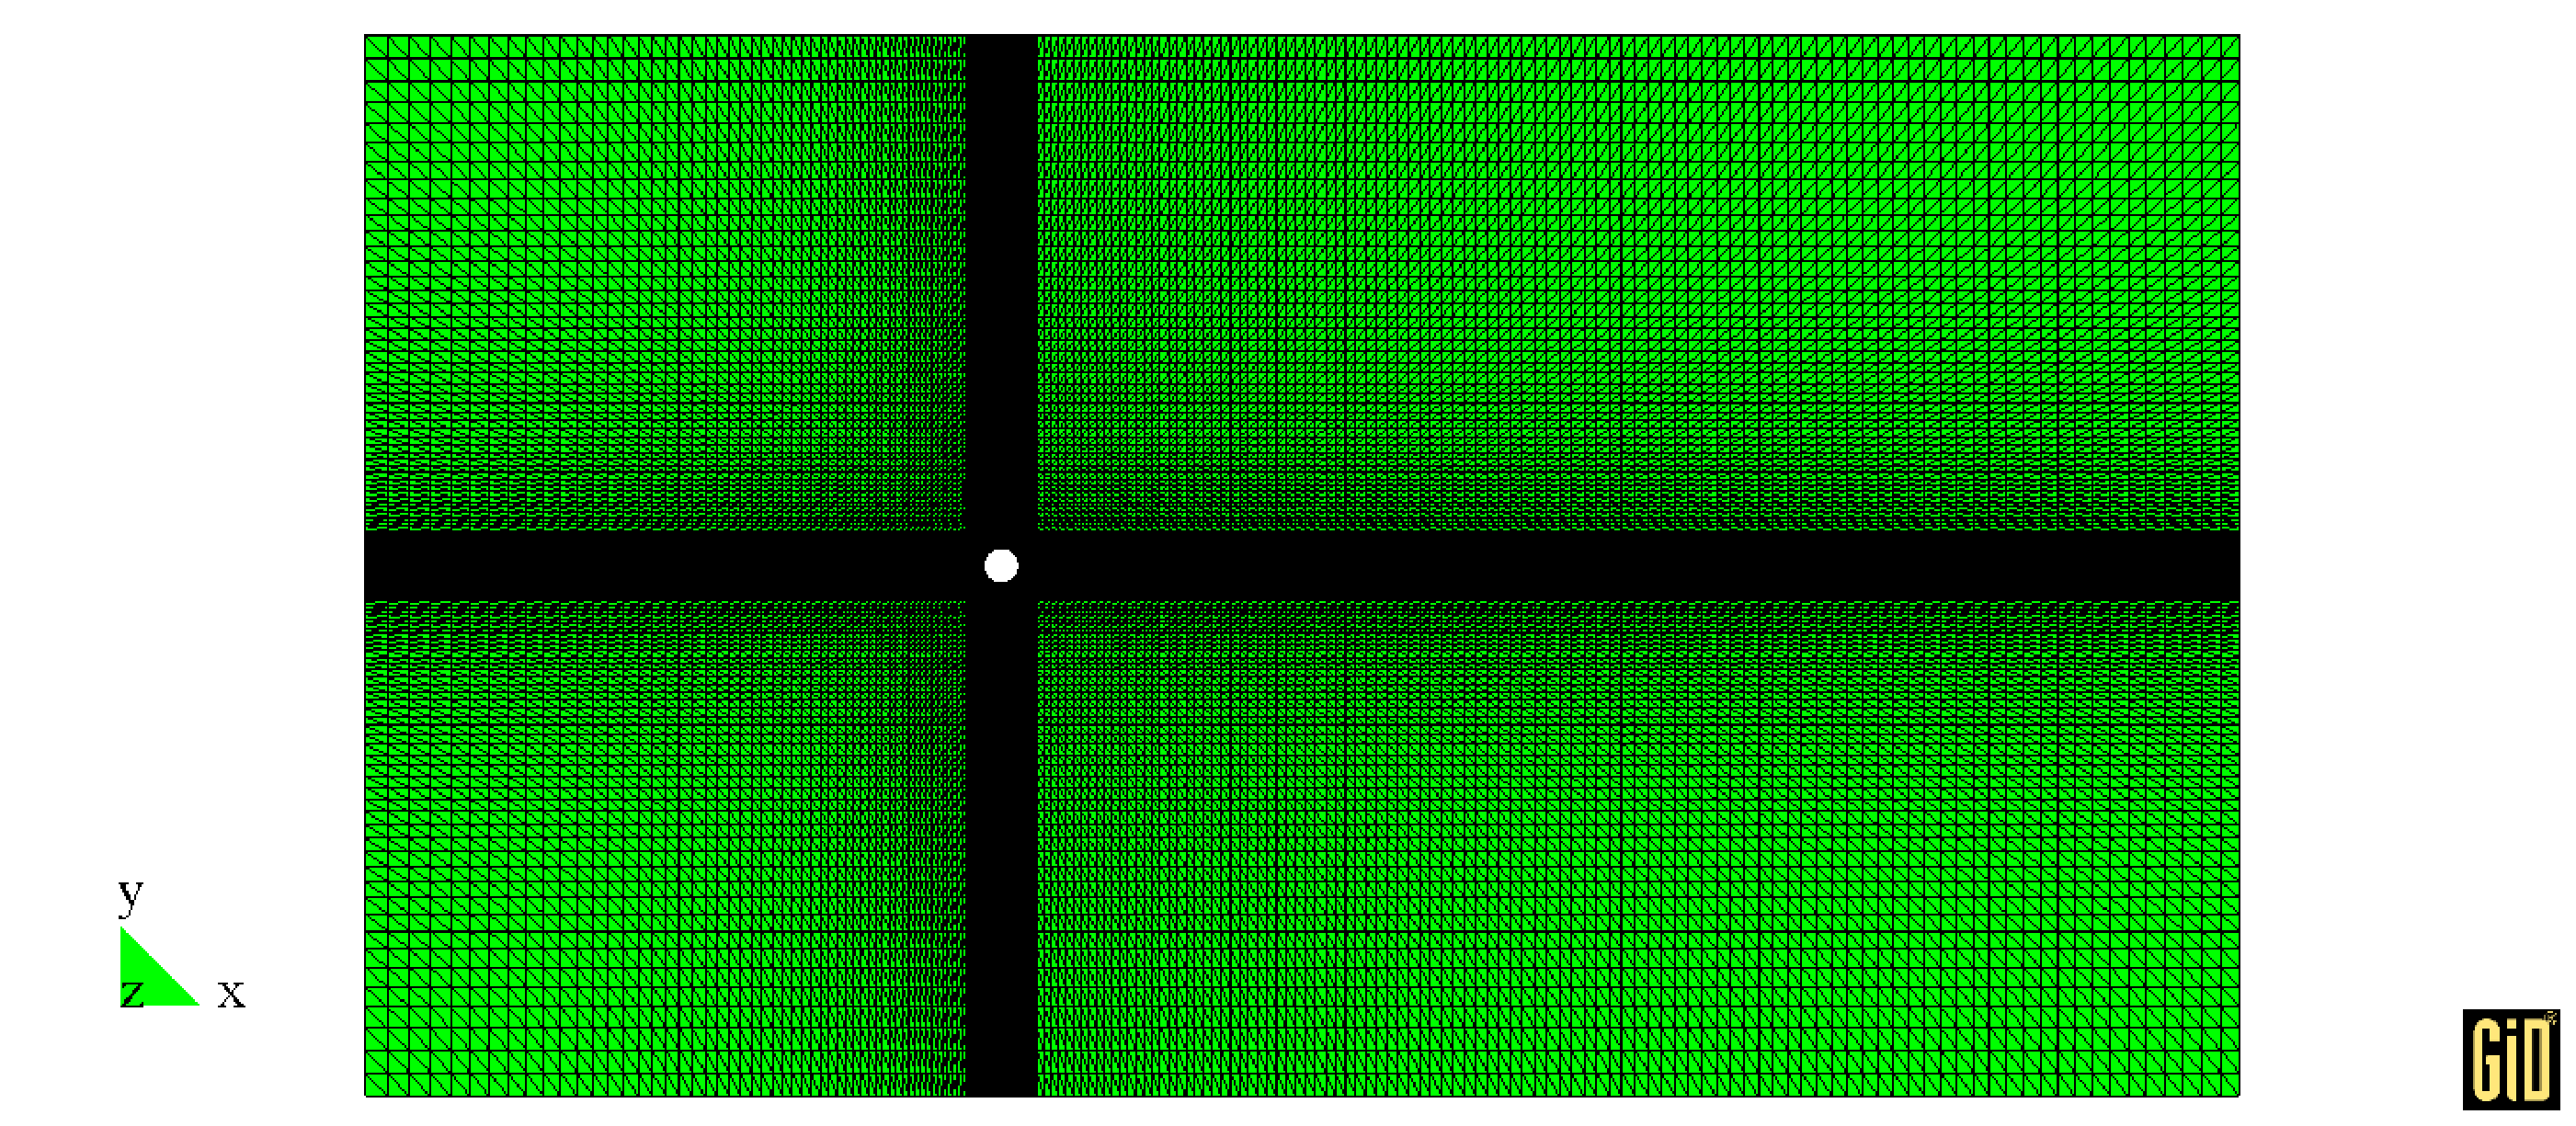
\includegraphics[width=6cm]{mesh.eps}
  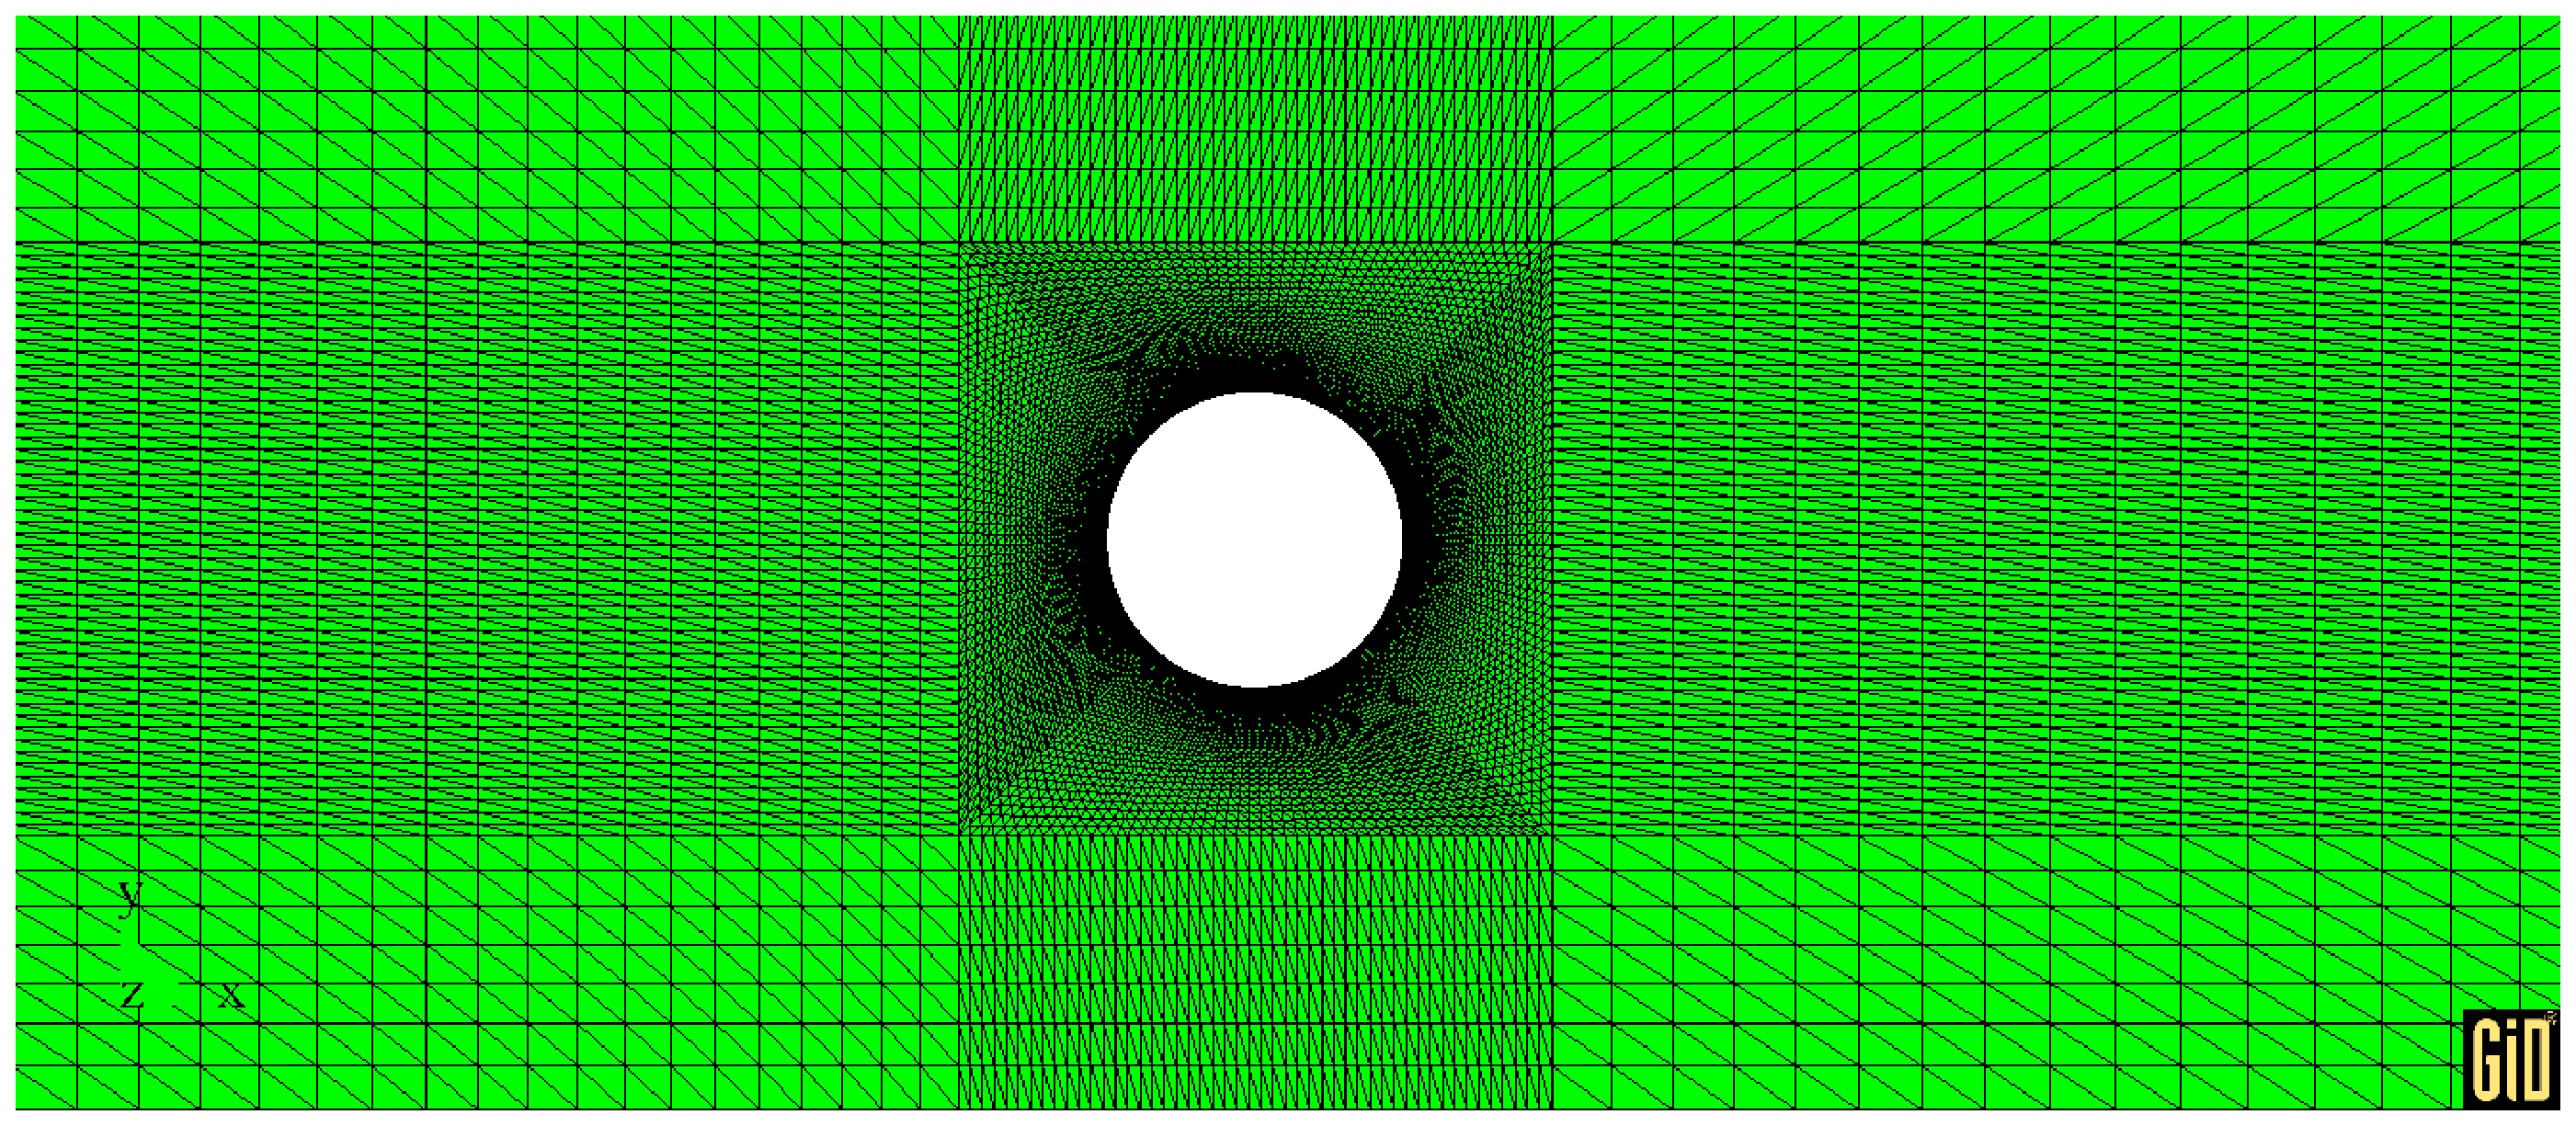
\includegraphics[width=6cm]{mesh_detail.eps}
  \end{center}
  \caption{General and detailed views of the mesh used for the baseflow computation and subsequent analysis, the circular cylinder is submerged a depth $h$.}
\end{figure}

%=====================================================================================
\section{Results}
\label{S:Results}
%=====================================================================================

The first thing to do is to search a steady state solution of the Navier-Stokes equations, for the space of parameters of the problem $Re,Fr,h/D$. In this letter we have analyzed a range of Reynolds numbers close to the first Hopf bifurcation that appears in the absence of free surface. This range is $Re=(30,70)$ while the Froude number has been kept fixed to $Fr=3$ and the water depth was $h=?$. The horizontal and vertical velocity components of the baseflow and the free surface position corresponding to the case $Re=45$ and $Fr=3$ are shown in figures \ref{f:baseflow} and \ref{f:VOF}.

\begin{figure}
\begin{center}
\label{f:baseflow}
  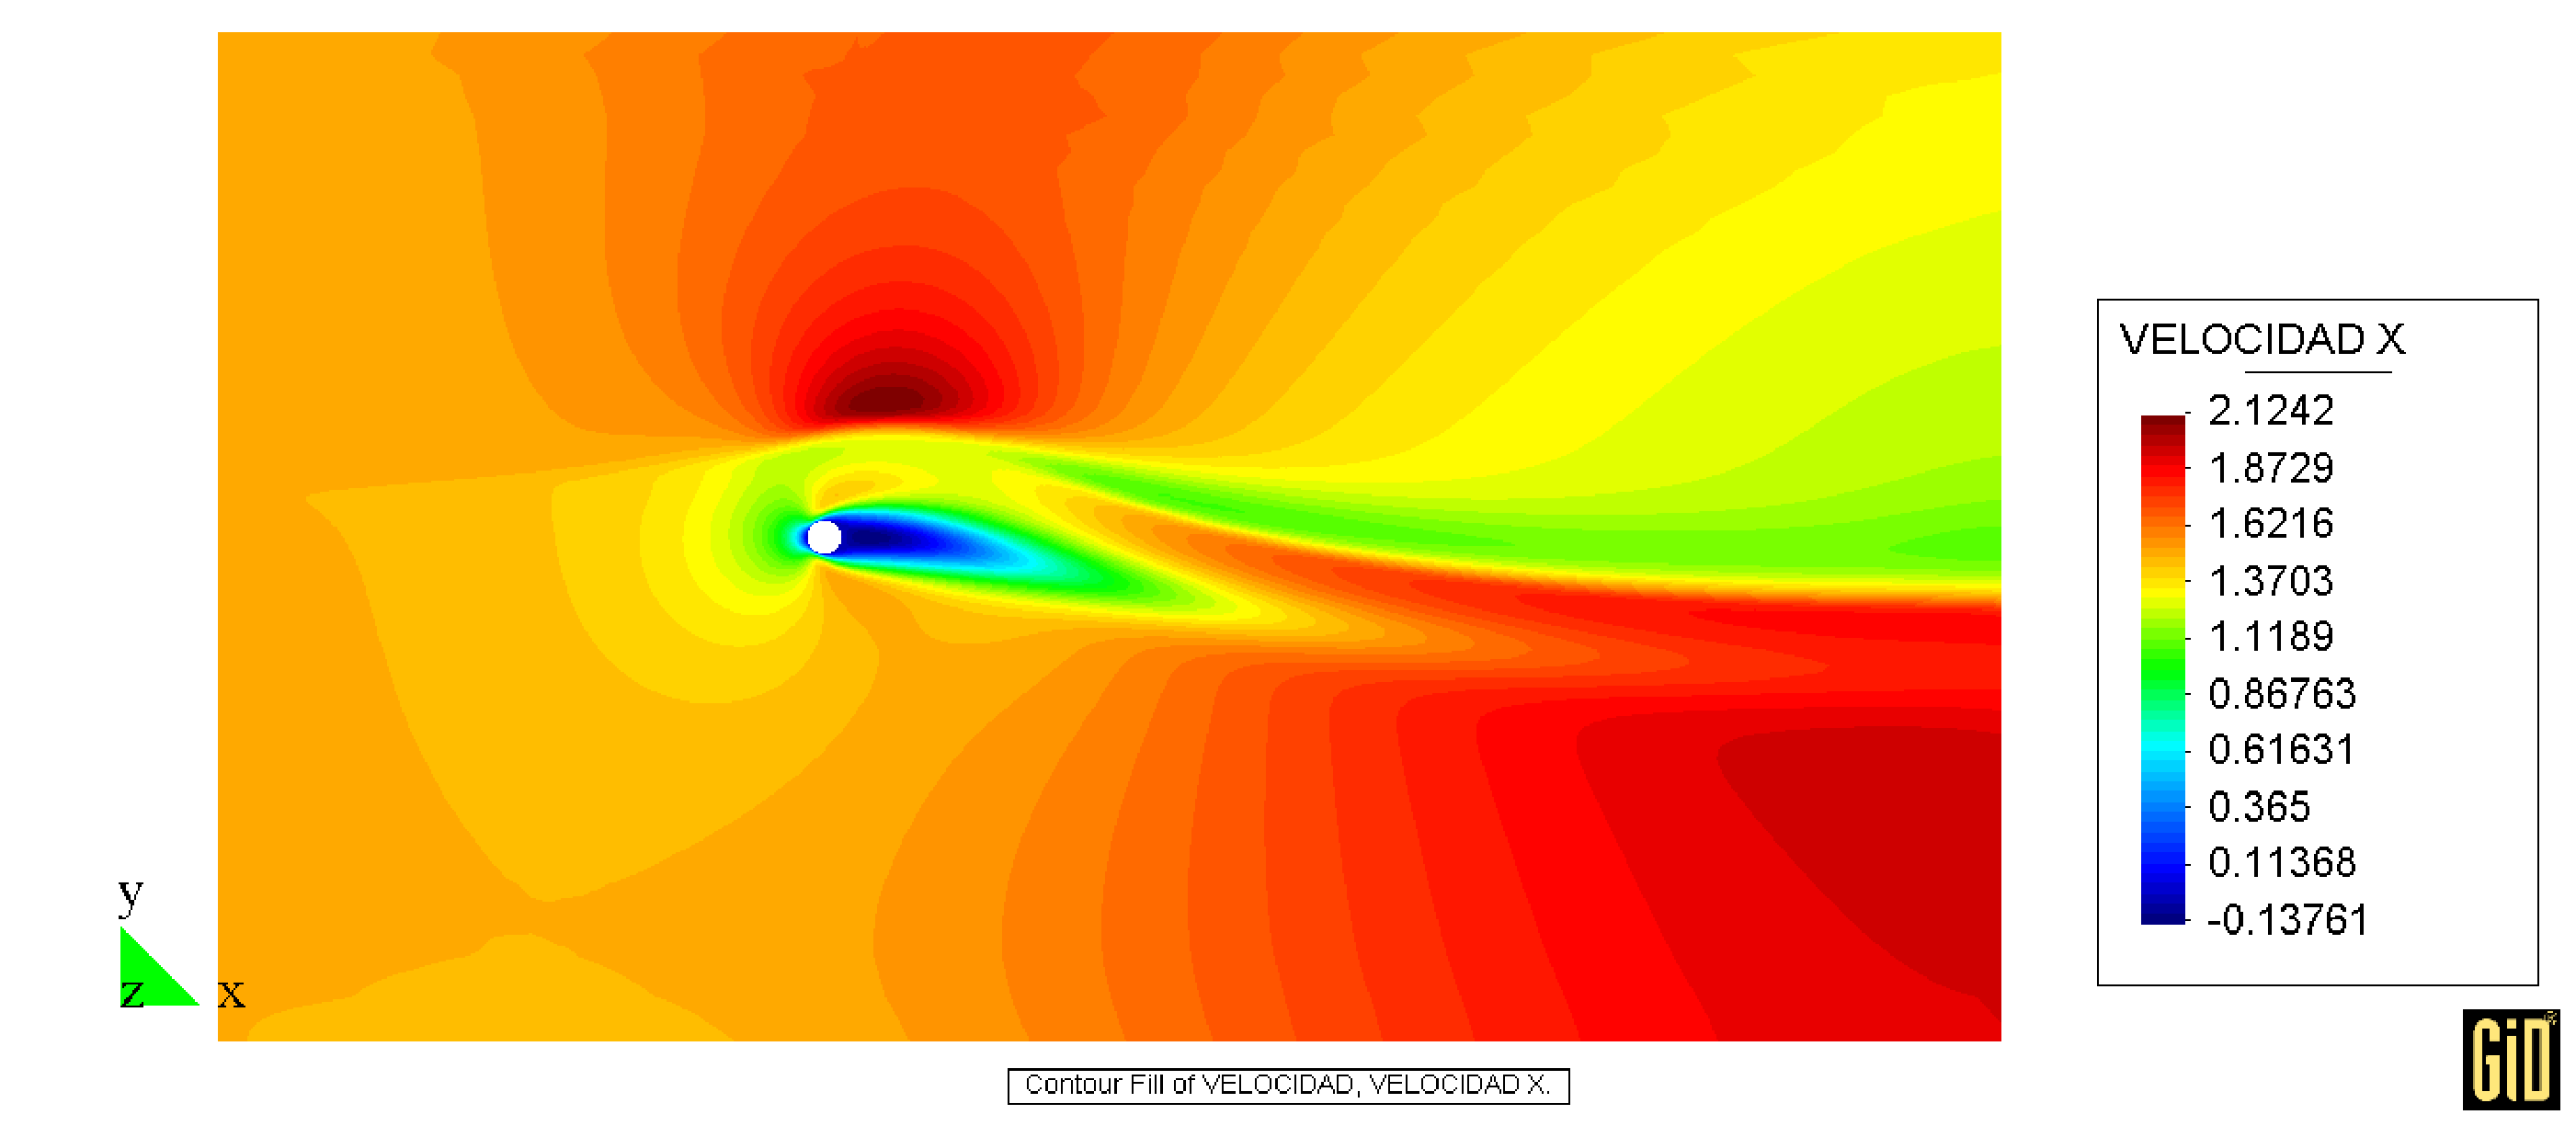
\includegraphics[width=6cm]{uRe45.eps}
  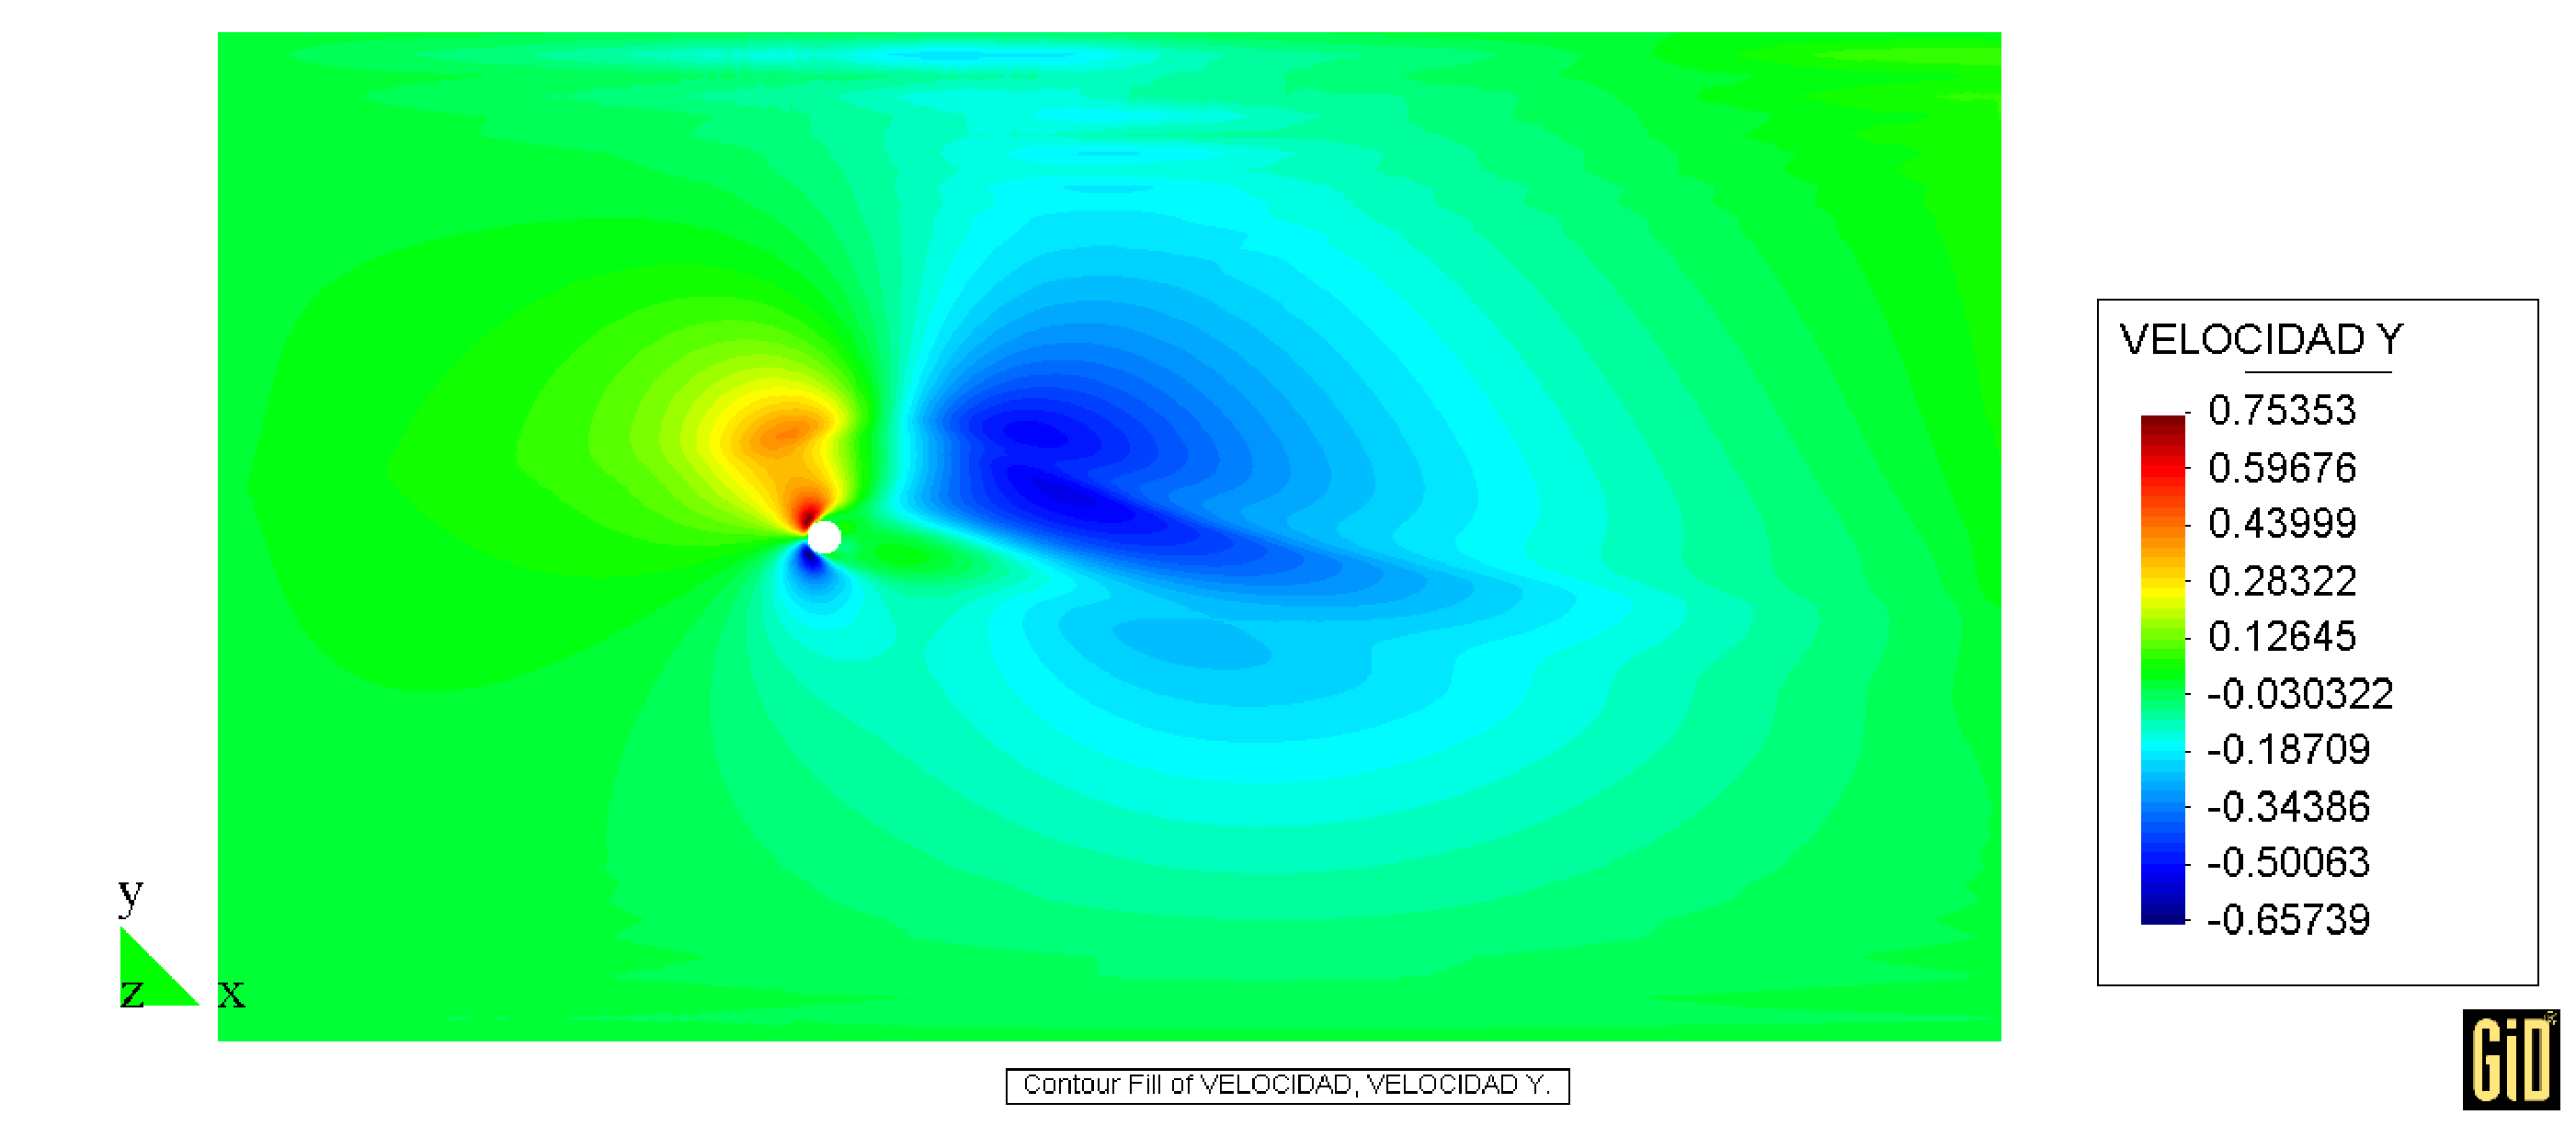
\includegraphics[width=6cm]{vRe45.eps}\\
  \end{center}
  \caption{Velocity representation at the steady state for $Re=45$ and $Fr=3$}
\end{figure}

 \begin{figure}
\begin{center}
\label{f:VOF}
  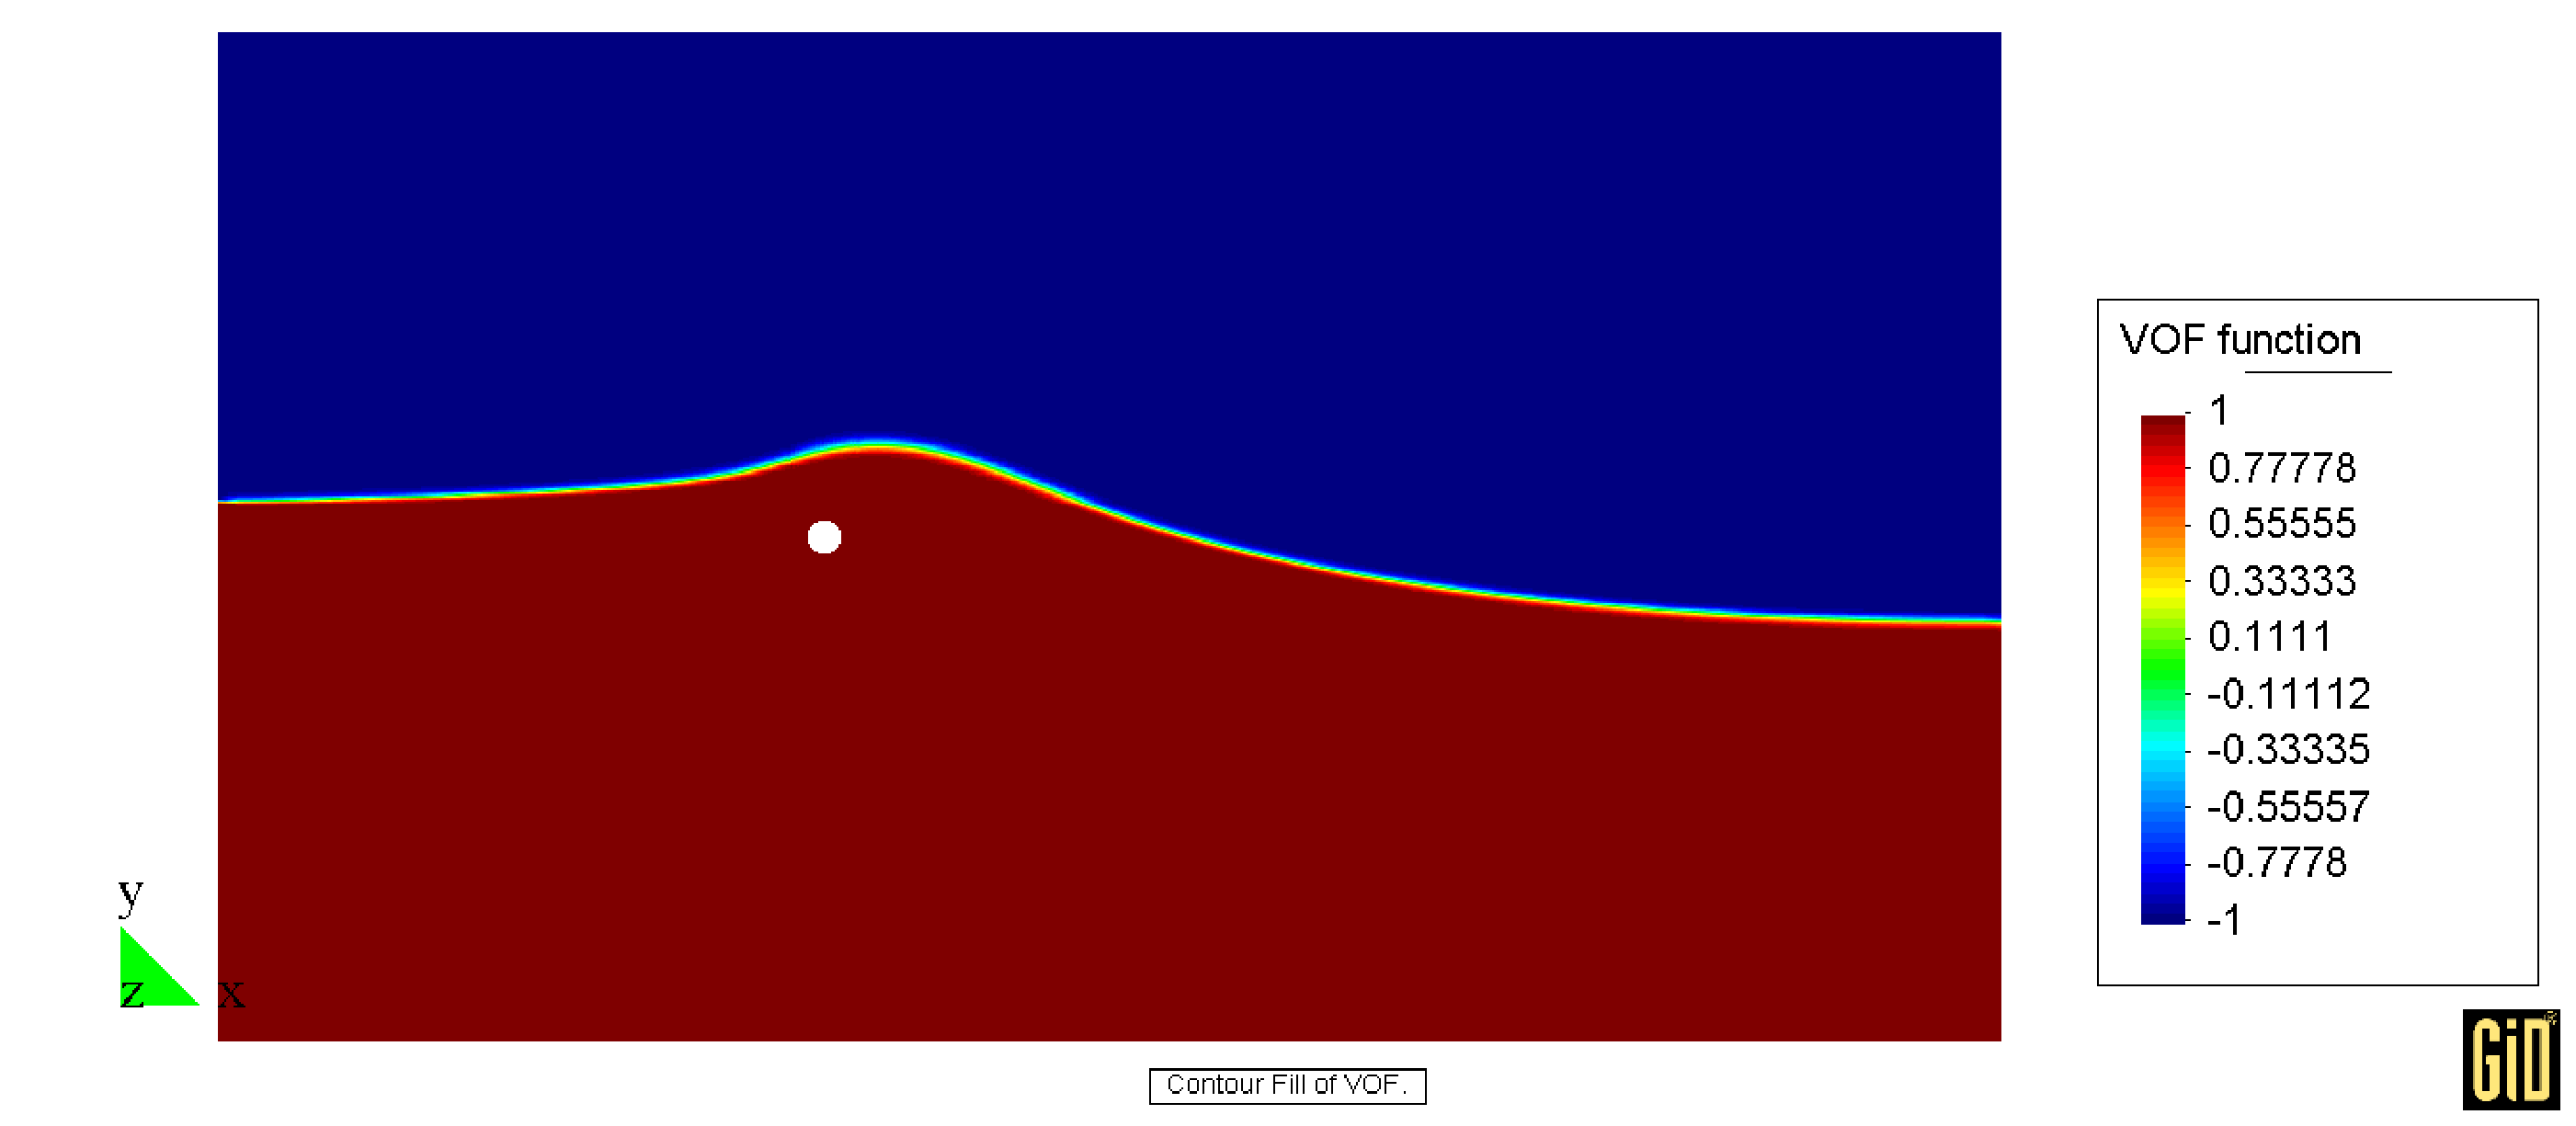
\includegraphics[width=6cm]{VOF.eps}\\
  \end{center}
  \caption{Free surface representation of the VOF scalar function at the steady state for $Re=45$ and $Fr=3$}
\end{figure}

\begin{figure}
\begin{center}
\label{f:CdCl}
  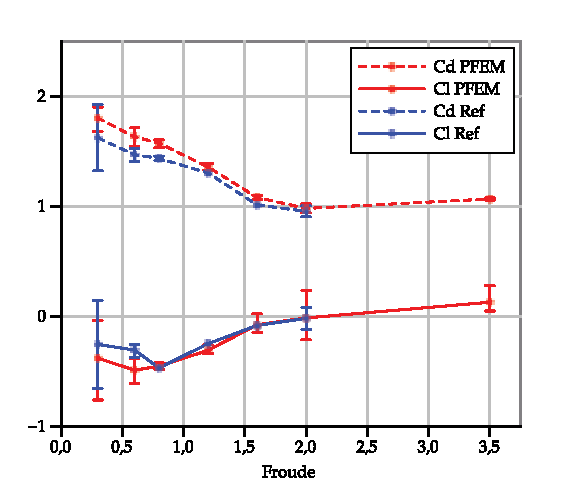
\includegraphics[width=6cm]{CdCl_Re180_hd_0_55.eps}\\
  \end{center}
  \caption{Drag and Lift coefficients calculated with PFEM-2 compared with the reference work of Bouscasse \cite{Bouscasse14}. $Re=180$.} %, $t^*=tU/d$.}
\end{figure}



A collection of steady baseflows has been obtained varying the Reynolds number for $Re=30,40,45,50,60,70$. For the sake of code validation, the global drag and lift forces have been compared against previous results\cite{Bouscasse} at the standard $Re=180$ and different Froude numbers being the agreement very satisfactory, see figure \ref{f:CdCl}. For each one a stability analysis based of the resolution of the large eigenvalue problem mentioned before has been done, and the evolution of the most unstable mode has been monitored. The evolution of the growth/damping rate and the angular frequencies of the most unstable mode for these Reynolds numbers is shown in figure \ref{f:omegas}. It can be observed that similarly to what happens in the absence of free surface the most unstable mode moves towards the unstable region $\omega_r<0$ when the Reynolds number is increased. For a Reynolds number very close to the one found in the absence of free surface $Re_c\approx 47$ the mode turns to be unstable a the vortex shedding appears in the flow. This frequency can be confirmed when the global force is monitored while the Navier-Stokes equations are solved, see figure \ref{f:lifts}. An increasing oscillation is appreciated once the critical Reynolds number $Re_c$ is exceeded. The novelty comes from the fact that the frequency associated to this oscillating unstable mode $\omega_= 0.98$ is higher when compared to the case without free surface aprox. 0.7. , this frequency shift implies that the mode oscillation is clearly accelerated by the presence of the free surface.


\begin{figure}
\begin{center}
\label{f:omegas}
  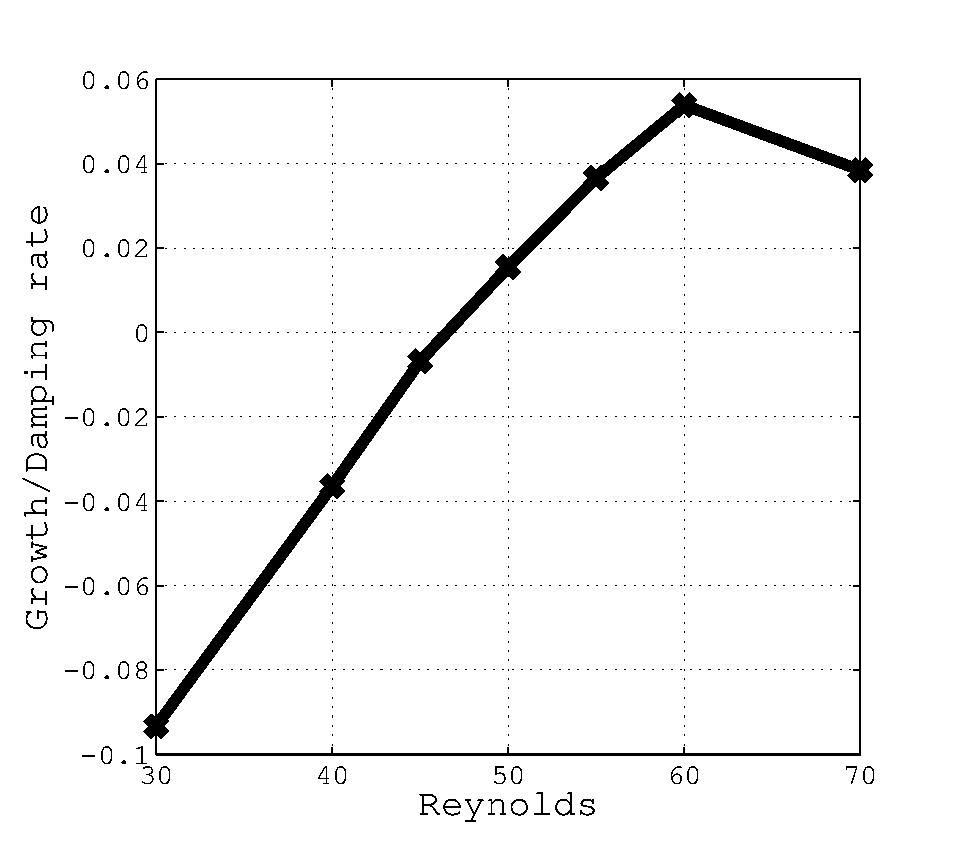
\includegraphics[width=5cm]{Growth.eps}
  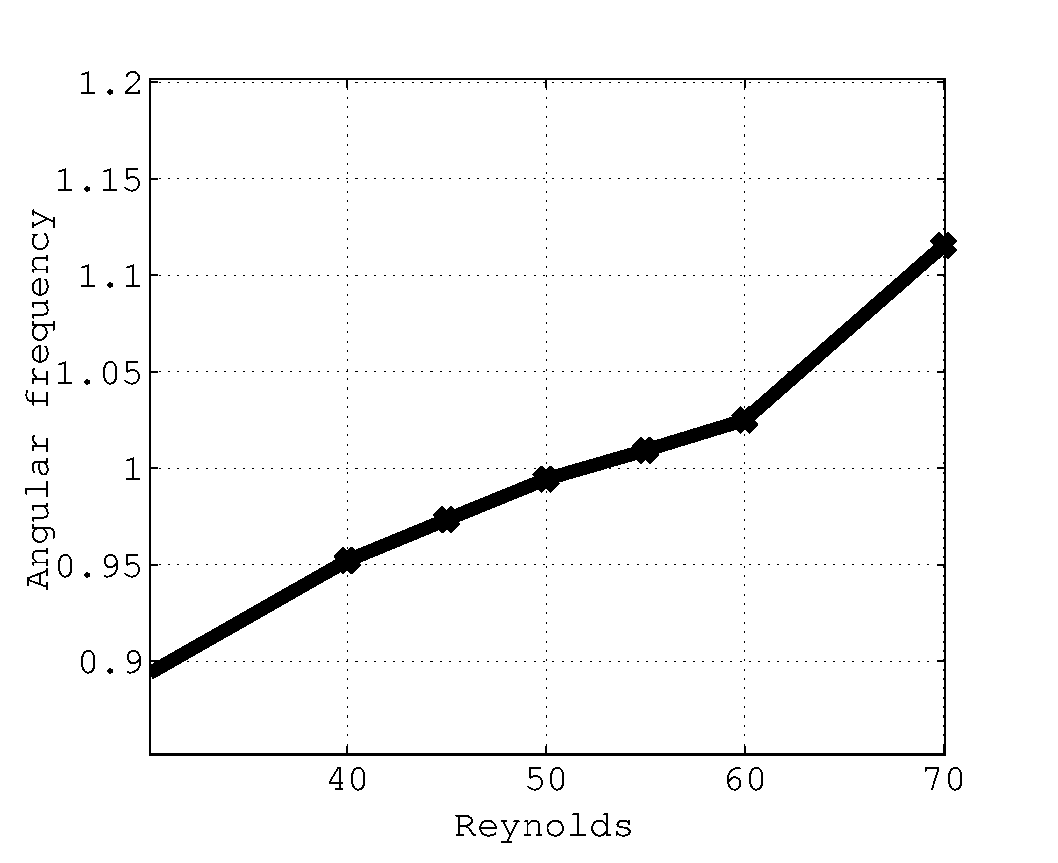
\includegraphics[width=5cm]{Freq.eps}\\
  \end{center}
  \caption{Growth rate $Fr=3$}
\end{figure}

\begin{figure}
\begin{center}
\label{f:lifts}
  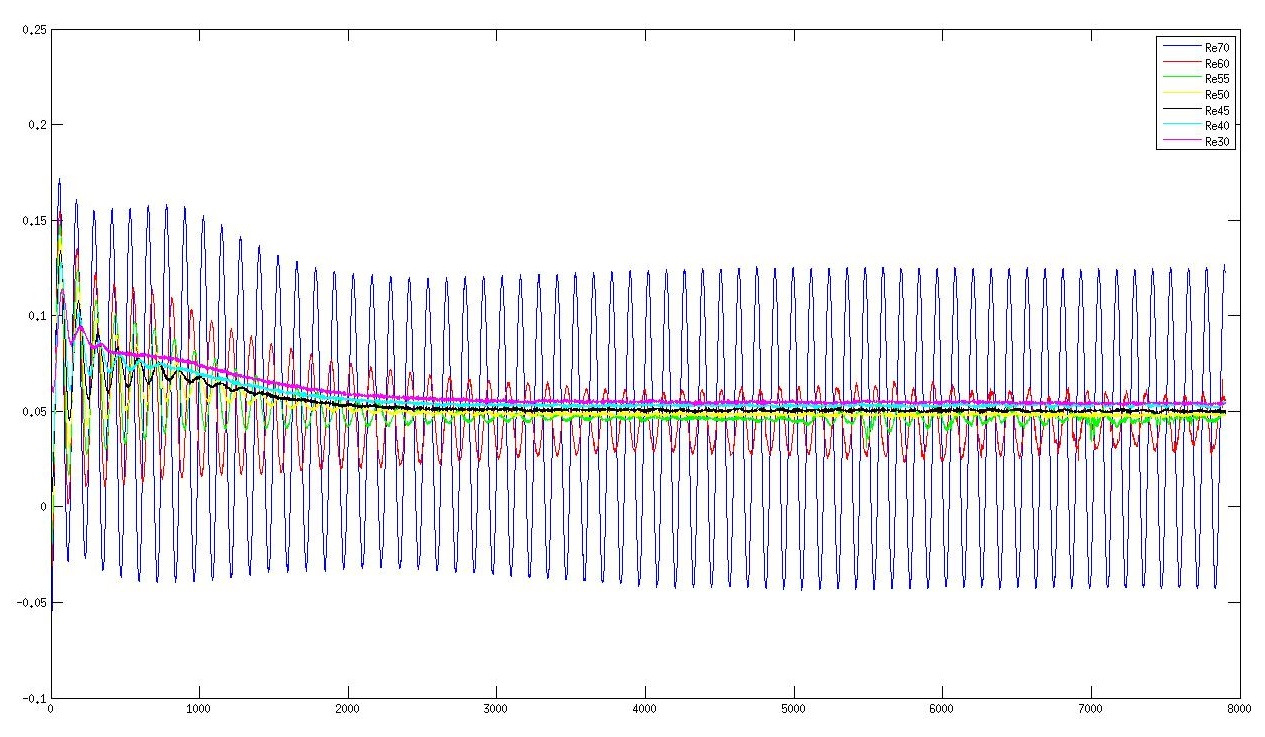
\includegraphics[width=6cm]{Cl_Fr3.0.eps}
  \end{center}
  \caption{Lift force at different Reynolds numbers.}
\end{figure}

The mode corresponding to this oscillating unstable mode is shown in figure \ref{f:mode}, where the shape of the mode follows the tendency described by the free surface position. 

   \begin{figure}
\begin{center}
\label{f:mode}
  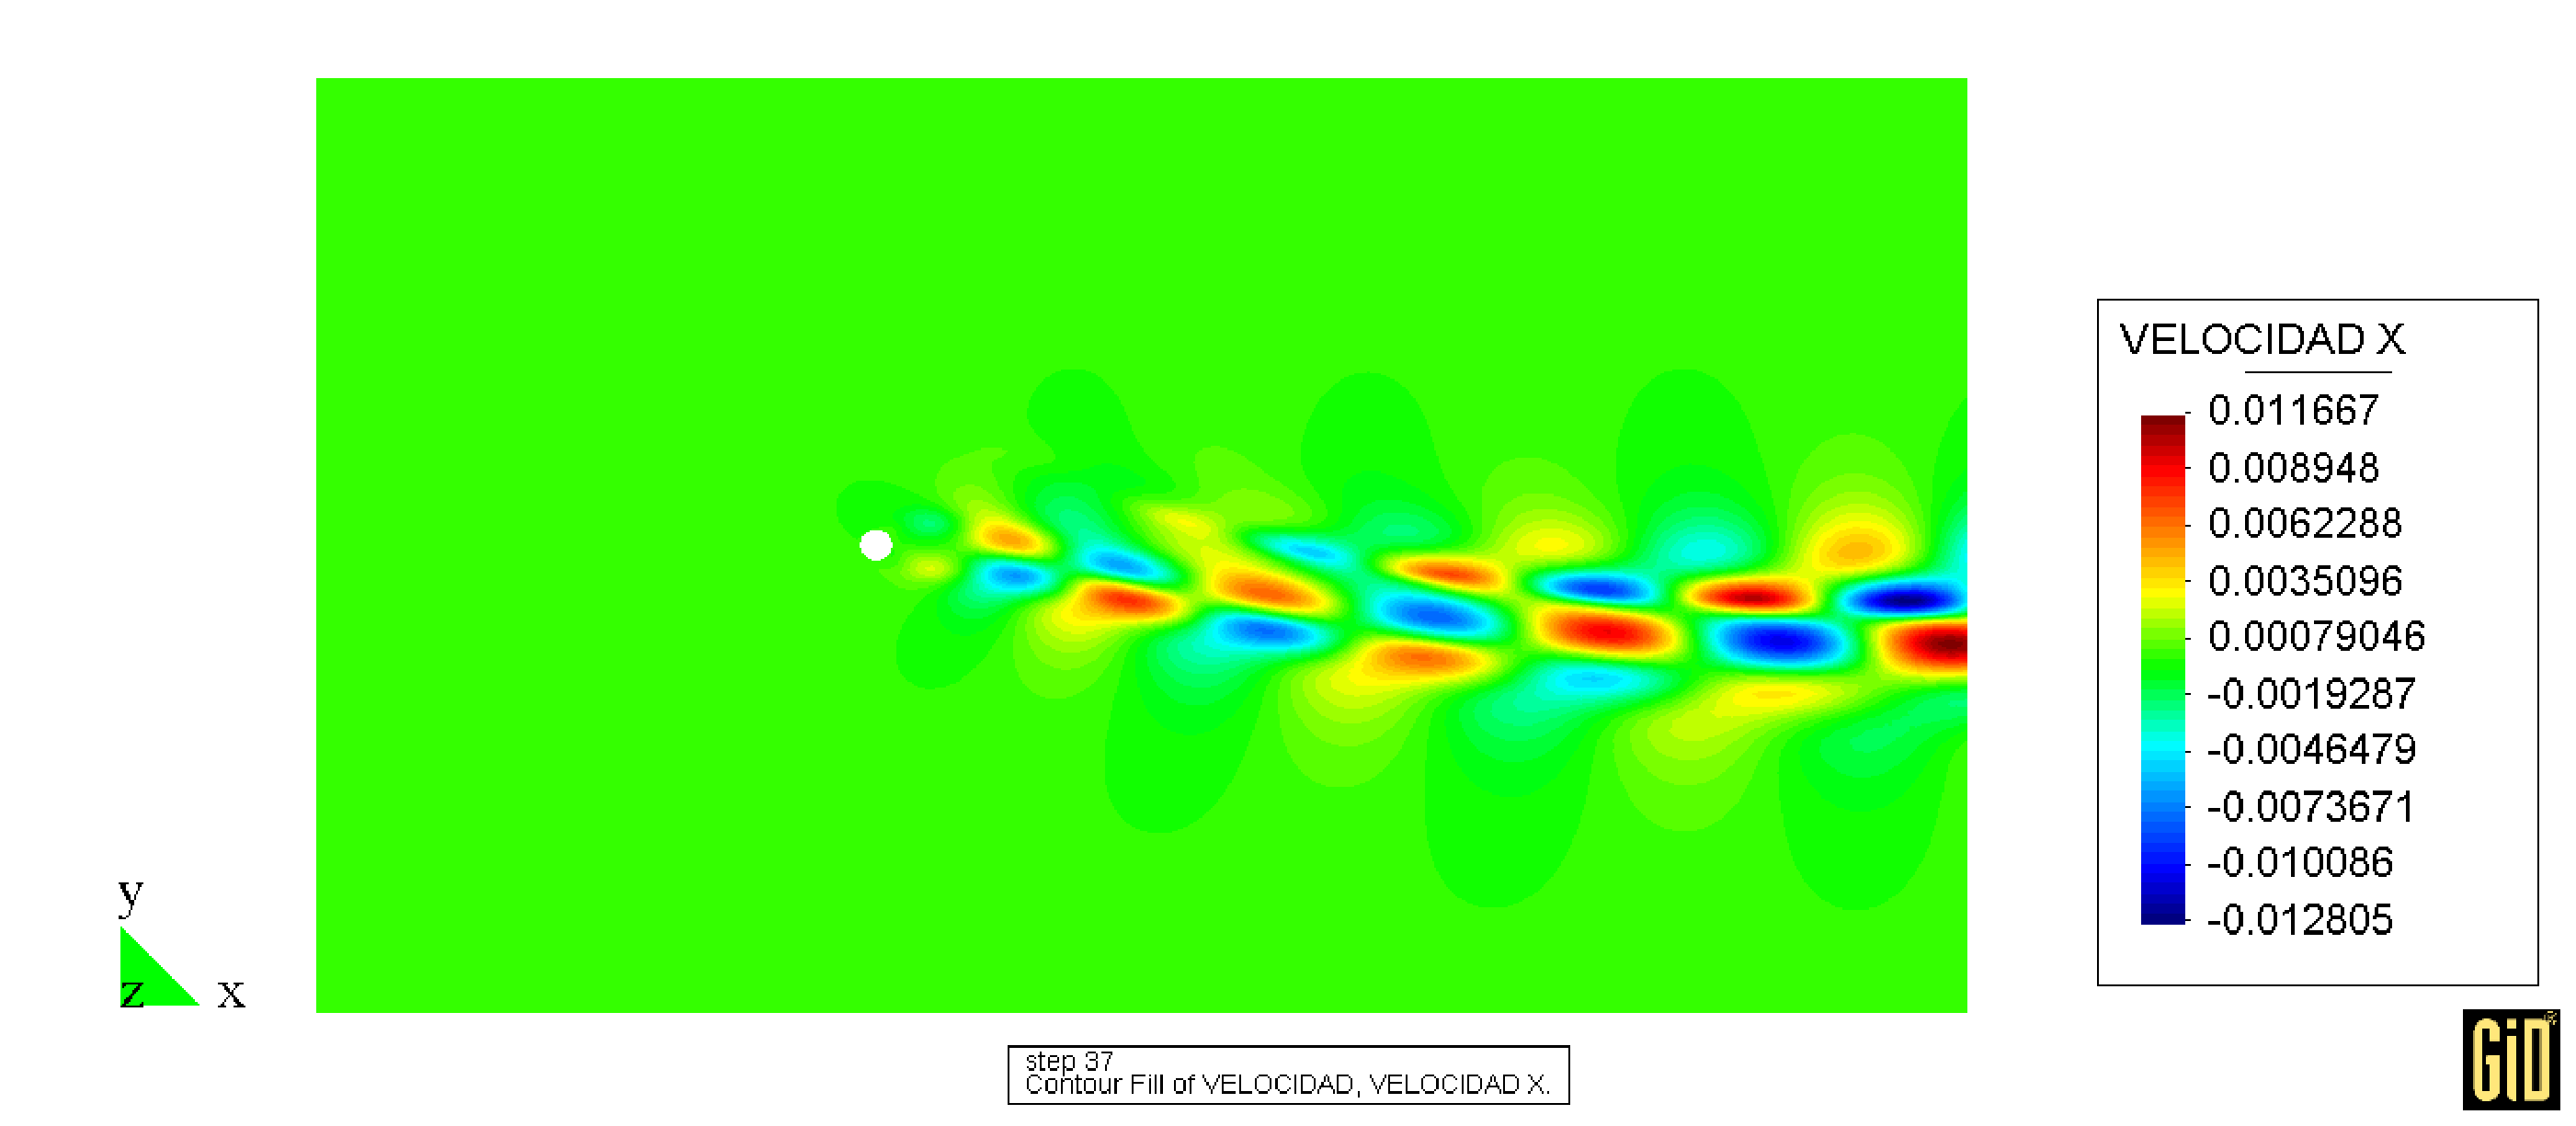
\includegraphics[width=6cm]{pertuRe45.eps}
  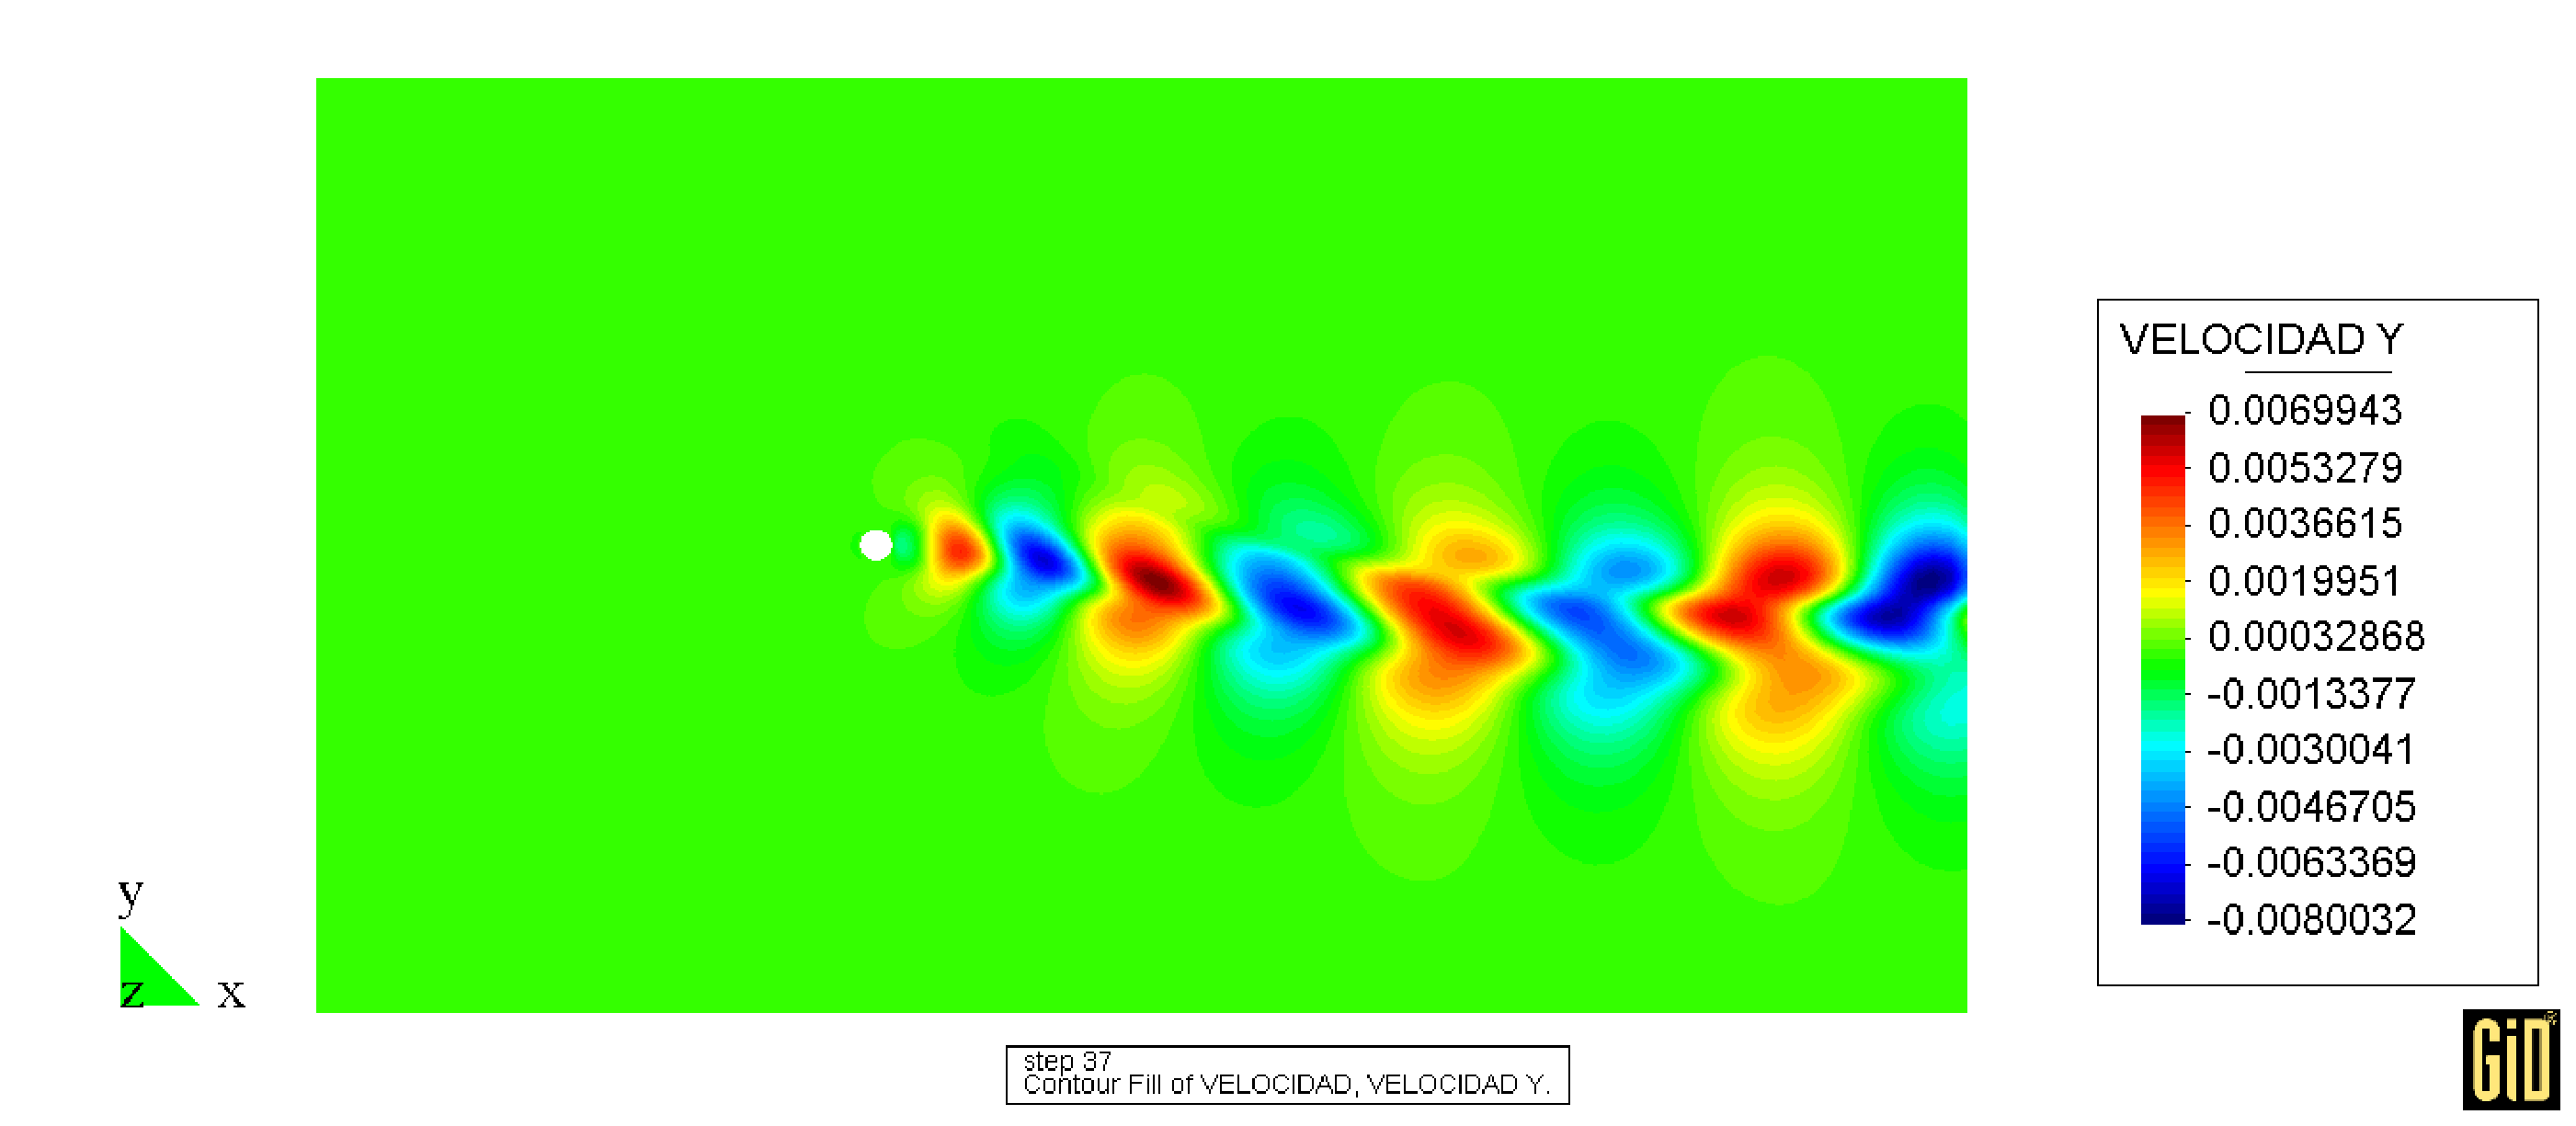
\includegraphics[width=6cm]{pertvRe45.eps}\\
  \end{center}
  \caption{Unstable mode $Re=45$ $Fr=3$}
\end{figure}


In the future these results will be also confirmed and extended to higher Reynolds values by a Dynamic Mode Decomposition. Also the possibility of having situations such that growing instabilities caused by the free surface oscillations could also included in the analysis, similar to what occurs in a Rayleigh-Taylor instability. The possibility will be studied in future works. 
It is believed that the theoretical findings of this Letter can be realized by experiments and confirmed by 3D simulations. This work was supported by the Technical University of Madrid by the project (PID) "Combination of Eulerian and Lagrangian methodologies for the solution of free surface flows."



Gonzalez
Idelhson
Williamson
[1] C. P. Jackson, J. Fluid Mech. 182, 23 (1987).
[2] C. Mathis, M. Provansal, and L. Boyer, J. Fluid Mech. 182, 1 (1987).
[3] C. H. K. Williamson, Phys. Fluids 31, 3165 (1988).
[4] G. D. Miller and C. H. K. Williamson, Exp. Fluid. 18, 26 (1994).



Biblio

\end{document} 